
%% bare_conf.tex
%% V1.3
%% 2007/01/11
%% by Michael Shell
%% See:
%% http://www.michaelshell.org/
%% for current contact information.
%%
%% This is a skeleton file demonstrating the use of IEEEtran.cls
%% (requires IEEEtran.cls version 1.7 or later) with an IEEE conference paper.
%%
%% Support sites:
%% http://www.michaelshell.org/tex/ieeetran/
%% http://www.ctan.org/tex-archive/macros/latex/contrib/IEEEtran/
%% and
%% http://www.ieee.org/

%%*************************************************************************
%% Legal Notice:
%% This code is offered as-is without any warranty either expressed or
%% implied; without even the implied warranty of MERCHANTABILITY or
%% FITNESS FOR A PARTICULAR PURPOSE! 
%% User assumes all risk.
%% In no event shall IEEE or any contributor to this code be liable for
%% any damages or losses, including, but not limited to, incidental,
%% consequential, or any other damages, resulting from the use or misuse
%% of any information contained here.
%%
%% All comments are the opinions of their respective authors and are not
%% necessarily endorsed by the IEEE.
%%
%% This work is distributed under the LaTeX Project Public License (LPPL)
%% ( http://www.latex-project.org/ ) version 1.3, and may be freely used,
%% distributed and modified. A copy of the LPPL, version 1.3, is included
%% in the base LaTeX documentation of all distributions of LaTeX released
%% 2003/12/01 or later.
%% Retain all contribution notices and credits.
%% ** Modified files should be clearly indicated as such, including  **
%% ** renaming them and changing author support contact information. **
%%
%% File list of work: IEEEtran.cls, IEEEtran_HOWTO.pdf, bare_adv.tex,
%%                    bare_conf.tex, bare_jrnl.tex, bare_jrnl_compsoc.tex
%%*************************************************************************

% *** Authors should verify (and, if needed, correct) their LaTeX system  ***
% *** with the testflow diagnostic prior to trusting their LaTeX platform ***
% *** with production work. IEEE's font choices can trigger bugs that do  ***
% *** not appear when using other class files.                            ***
% The testflow support page is at:
% http://www.michaelshell.org/tex/testflow/



% Note that the a4paper option is mainly intended so that authors in
% countries using A4 can easily print to A4 and see how their papers will
% look in print - the typesetting of the document will not typically be
% affected with changes in paper size (but the bottom and side margins will).
% Use the testflow package mentioned above to verify correct handling of
% both paper sizes by the user's LaTeX system.
%
% Also note that the "draftcls" or "draftclsnofoot", not "draft", option
% should be used if it is desired that the figures are to be displayed in
% draft mode.
%
\documentclass[conference]{IEEEtran}
% Add the compsoc option for Computer Society conferences.
%
% If IEEEtran.cls has not been installed into the LaTeX system files,
% manually specify the path to it like:
% \documentclass[conference]{../sty/IEEEtran}





% Some very useful LaTeX packages include:
% (uncomment the ones you want to load)


% *** MISC UTILITY PACKAGES ***
%
%\usepackage{ifpdf}
% Heiko Oberdiek's ifpdf.sty is very useful if you need conditional
% compilation based on whether the output is pdf or dvi.
% usage:
% \ifpdf
%   % pdf code
% \else
%   % dvi code
% \fi
% The latest version of ifpdf.sty can be obtained from:
% http://www.ctan.org/tex-archive/macros/latex/contrib/oberdiek/
% Also, note that IEEEtran.cls V1.7 and later provides a builtin
% \ifCLASSINFOpdf conditional that works the same way.
% When switching from latex to pdflatex and vice-versa, the compiler may
% have to be run twice to clear warning/error messages.






% *** CITATION PACKAGES ***
%
%\usepackage{cite}
% cite.sty was written by Donald Arseneau
% V1.6 and later of IEEEtran pre-defines the format of the cite.sty package
% \cite{} output to follow that of IEEE. Loading the cite package will
% result in citation numbers being automatically sorted and properly
% "compressed/ranged". e.g., [1], [9], [2], [7], [5], [6] without using
% cite.sty will become [1], [2], [5]--[7], [9] using cite.sty. cite.sty's
% \cite will automatically add leading space, if needed. Use cite.sty's
% noadjust option (cite.sty V3.8 and later) if you want to turn this off.
% cite.sty is already installed on most LaTeX systems. Be sure and use
% version 4.0 (2003-05-27) and later if using hyperref.sty. cite.sty does
% not currently provide for hyperlinked citations.
% The latest version can be obtained at:
% http://www.ctan.org/tex-archive/macros/latex/contrib/cite/
% The documentation is contained in the cite.sty file itself.






% *** GRAPHICS RELATED PACKAGES ***
%
\ifCLASSINFOpdf
  % \usepackage[pdftex]{graphicx}
  % declare the path(s) where your graphic files are
  % \graphicspath{{../pdf/}{../jpeg/}}
  % and their extensions so you won't have to specify these with
  % every instance of \includegraphics
  % \DeclareGraphicsExtensions{.pdf,.jpeg,.png}
\else
  % or other class option (dvipsone, dvipdf, if not using dvips). graphicx
  % will default to the driver specified in the system graphics.cfg if no
  % driver is specified.
  % \usepackage[dvips]{graphicx}
  % declare the path(s) where your graphic files are
  % \graphicspath{{../eps/}}
  % and their extensions so you won't have to specify these with
  % every instance of \includegraphics
  % \DeclareGraphicsExtensions{.eps}
\fi
% graphicx was written by David Carlisle and Sebastian Rahtz. It is
% required if you want graphics, photos, etc. graphicx.sty is already
% installed on most LaTeX systems. The latest version and documentation can
% be obtained at: 
% http://www.ctan.org/tex-archive/macros/latex/required/graphics/
% Another good source of documentation is "Using Imported Graphics in
% LaTeX2e" by Keith Reckdahl which can be found as epslatex.ps or
% epslatex.pdf at: http://www.ctan.org/tex-archive/info/
%
% latex, and pdflatex in dvi mode, support graphics in encapsulated
% postscript (.eps) format. pdflatex in pdf mode supports graphics
% in .pdf, .jpeg, .png and .mps (metapost) formats. Users should ensure
% that all non-photo figures use a vector format (.eps, .pdf, .mps) and
% not a bitmapped formats (.jpeg, .png). IEEE frowns on bitmapped formats
% which can result in "jaggedy"/blurry rendering of lines and letters as
% well as large increases in file sizes.
%
% You can find documentation about the pdfTeX application at:
% http://www.tug.org/applications/pdftex





% *** MATH PACKAGES ***
%
%\usepackage[cmex10]{amsmath}
% A popular package from the American Mathematical Society that provides
% many useful and powerful commands for dealing with mathematics. If using
% it, be sure to load this package with the cmex10 option to ensure that
% only type 1 fonts will utilized at all point sizes. Without this option,
% it is possible that some math symbols, particularly those within
% footnotes, will be rendered in bitmap form which will result in a
% document that can not be IEEE Xplore compliant!
%
% Also, note that the amsmath package sets \interdisplaylinepenalty to 10000
% thus preventing page breaks from occurring within multiline equations. Use:
%\interdisplaylinepenalty=2500
% after loading amsmath to restore such page breaks as IEEEtran.cls normally
% does. amsmath.sty is already installed on most LaTeX systems. The latest
% version and documentation can be obtained at:
% http://www.ctan.org/tex-archive/macros/latex/required/amslatex/math/





% *** SPECIALIZED LIST PACKAGES ***
%
%\usepackage{algorithmic}
% algorithmic.sty was written by Peter Williams and Rogerio Brito.
% This package provides an algorithmic environment fo describing algorithms.
% You can use the algorithmic environment in-text or within a figure
% environment to provide for a floating algorithm. Do NOT use the algorithm
% floating environment provided by algorithm.sty (by the same authors) or
% algorithm2e.sty (by Christophe Fiorio) as IEEE does not use dedicated
% algorithm float types and packages that provide these will not provide
% correct IEEE style captions. The latest version and documentation of
% algorithmic.sty can be obtained at:
% http://www.ctan.org/tex-archive/macros/latex/contrib/algorithms/
% There is also a support site at:
% http://algorithms.berlios.de/index.html
% Also of interest may be the (relatively newer and more customizable)
% algorithmicx.sty package by Szasz Janos:
% http://www.ctan.org/tex-archive/macros/latex/contrib/algorithmicx/




% *** ALIGNMENT PACKAGES ***
%
%\usepackage{array}
% Frank Mittelbach's and David Carlisle's array.sty patches and improves
% the standard LaTeX2e array and tabular environments to provide better
% appearance and additional user controls. As the default LaTeX2e table
% generation code is lacking to the point of almost being broken with
% respect to the quality of the end results, all users are strongly
% advised to use an enhanced (at the very least that provided by array.sty)
% set of table tools. array.sty is already installed on most systems. The
% latest version and documentation can be obtained at:
% http://www.ctan.org/tex-archive/macros/latex/required/tools/


%\usepackage{mdwmath}
%\usepackage{mdwtab}
% Also highly recommended is Mark Wooding's extremely powerful MDW tools,
% especially mdwmath.sty and mdwtab.sty which are used to format equations
% and tables, respectively. The MDWtools set is already installed on most
% LaTeX systems. The lastest version and documentation is available at:
% http://www.ctan.org/tex-archive/macros/latex/contrib/mdwtools/


% IEEEtran contains the IEEEeqnarray family of commands that can be used to
% generate multiline equations as well as matrices, tables, etc., of high
% quality.


%\usepackage{eqparbox}
% Also of notable interest is Scott Pakin's eqparbox package for creating
% (automatically sized) equal width boxes - aka "natural width parboxes".
% Available at:
% http://www.ctan.org/tex-archive/macros/latex/contrib/eqparbox/





% *** SUBFIGURE PACKAGES ***
\usepackage[tight,footnotesize]{subfigure}
% subfigure.sty was written by Steven Douglas Cochran. This package makes it
% easy to put subfigures in your figures. e.g., "Figure 1a and 1b". For IEEE
% work, it is a good idea to load it with the tight package option to reduce
% the amount of white space around the subfigures. subfigure.sty is already
% installed on most LaTeX systems. The latest version and documentation can
% be obtained at:
% http://www.ctan.org/tex-archive/obsolete/macros/latex/contrib/subfigure/
% subfigure.sty has been superceeded by subfig.sty.



%\usepackage[caption=false]{caption}
%\usepackage[font=footnotesize]{subfig}
% subfig.sty, also written by Steven Douglas Cochran, is the modern
% replacement for subfigure.sty. However, subfig.sty requires and
% automatically loads Axel Sommerfeldt's caption.sty which will override
% IEEEtran.cls handling of captions and this will result in nonIEEE style
% figure/table captions. To prevent this problem, be sure and preload
% caption.sty with its "caption=false" package option. This is will preserve
% IEEEtran.cls handing of captions. Version 1.3 (2005/06/28) and later 
% (recommended due to many improvements over 1.2) of subfig.sty supports
% the caption=false option directly:
%\usepackage[caption=false,font=footnotesize]{subfig}
%
% The latest version and documentation can be obtained at:
% http://www.ctan.org/tex-archive/macros/latex/contrib/subfig/
% The latest version and documentation of caption.sty can be obtained at:
% http://www.ctan.org/tex-archive/macros/latex/contrib/caption/




% *** FLOAT PACKAGES ***
%
%\usepackage{fixltx2e}
% fixltx2e, the successor to the earlier fix2col.sty, was written by
% Frank Mittelbach and David Carlisle. This package corrects a few problems
% in the LaTeX2e kernel, the most notable of which is that in current
% LaTeX2e releases, the ordering of single and double column floats is not
% guaranteed to be preserved. Thus, an unpatched LaTeX2e can allow a
% single column figure to be placed prior to an earlier double column
% figure. The latest version and documentation can be found at:
% http://www.ctan.org/tex-archive/macros/latex/base/



\usepackage{stfloats}
% stfloats.sty was written by Sigitas Tolusis. This package gives LaTeX2e
% the ability to do double column floats at the bottom of the page as well
% as the top. (e.g., "\begin{figure*}[!b]" is not normally possible in
% LaTeX2e). It also provides a command:
%\fnbelowfloat
% to enable the placement of footnotes below bottom floats (the standard
% LaTeX2e kernel puts them above bottom floats). This is an invasive package
% which rewrites many portions of the LaTeX2e float routines. It may not work
% with other packages that modify the LaTeX2e float routines. The latest
% version and documentation can be obtained at:
% http://www.ctan.org/tex-archive/macros/latex/contrib/sttools/
% Documentation is contained in the stfloats.sty comments as well as in the
% presfull.pdf file. Do not use the stfloats baselinefloat ability as IEEE
% does not allow \baselineskip to stretch. Authors submitting work to the
% IEEE should note that IEEE rarely uses double column equations and
% that authors should try to avoid such use. Do not be tempted to use the
% cuted.sty or midfloat.sty packages (also by Sigitas Tolusis) as IEEE does
% not format its papers in such ways.





% *** PDF, URL AND HYPERLINK PACKAGES ***
%
%\usepackage{url}
% url.sty was written by Donald Arseneau. It provides better support for
% handling and breaking URLs. url.sty is already installed on most LaTeX
% systems. The latest version can be obtained at:
% http://www.ctan.org/tex-archive/macros/latex/contrib/misc/
% Read the url.sty source comments for usage information. Basically,
% \url{my_url_here}.





% *** Do not adjust lengths that control margins, column widths, etc. ***
% *** Do not use packages that alter fonts (such as pslatex).         ***
% There should be no need to do such things with IEEEtran.cls V1.6 and later.
% (Unless specifically asked to do so by the journal or conference you plan
% to submit to, of course. )


% correct bad hyphenation here
\hyphenation{op-tical net-works semi-conduc-tor}

\usepackage[pdftex]{graphicx}

\begin{document}



\DeclareGraphicsExtensions{.pdf,.jpeg,.png,.jpg}

\newenvironment{figura}
  {\def\@captype{figure}}
  {}
\makeatother
%
% paper title
% can use linebreaks \\ within to get better formatting as desired
\title{NFAuthenticator: the key is your phone}


% author names and affiliations
% use a multiple column layout for up to three different
% affiliations
\author{\IEEEauthorblockN{Daniele Ronzani}
\IEEEauthorblockA{Department of Mathematics\\
University of Padua\\
Padua, Italy\\
daniele.ronzani@gmail.com}
\and
\IEEEauthorblockN{Michele Massaro}
\IEEEauthorblockA{Department of Mathematics\\
University of Padua\\
Padua, Italy\\
michele.massaro@me.com}}

% conference papers do not typically use \thanks and this command
% is locked out in conference mode. If realizereally needed, such as for
% the acknowledgment of grants, issue a \IEEEoverridecommandlockouts
% after \documentclass

% for over three affiliations, or if they all won't fit within the width
% of the page, use this alternative format:
% 
%\author{\IEEEauthorblockN{Michael Shell\IEEEauthorrefmark{1},
%Homer Simpson\IEEEauthorrefmark{2},
%James Kirk\IEEEauthorrefmark{3}, 
%Montgomery Scott\IEEEauthorrefmark{3} and
%Eldon Tyrell\IEEEauthorrefmark{4}}
%\IEEEauthorblockA{\IEEEauthorrefmark{1}School of Electrical and Computer Engineering\\
%Georgia Institute of Technology,
%Atlanta, Georgia 30332--0250\\ Email: see http://www.michaelshell.org/contact.html}
%\IEEEauthorblockA{\IEEEauthorrefmark{2}Twentieth Century Fox, Springfield, USA\\
%Email: homer@thesimpsons.com}
%\IEEEauthorblockA{\IEEEauthorrefmark{3}Starfleet Academy, San Francisco, California 96678-2391\\
%Telephone: (800) 555--1212, Fax: (888) 555--1212}
%\IEEEauthorblockA{\IEEEauthorrefmark{4}Tyrell Inc., 123 Replicant Street, Los Angeles, California 90210--4321}}




% use for special paper notices
%\IEEEspecialpapernotice{(Invited Paper)}




% make the title area
\maketitle


\begin{abstract}
%\boldmath
NFC is a technology that allows communication over short distance. Nowadays it is used to exchange data between smartphone or for authentication system, for example many buildings use tags instead of keys to open doors.
Actually, most of the current solutions are based on the identification of the user using the information contained inside the NFC tag.
This approach implies some problems involved by the use of a passive key, such as the inability to lock the key to prevent unauthorized use.
The purpose of this work is to create an authentication system based on a client-server architecture that allows to access, through a login, to some areas inside a building identified by NFC tags and read by an Android phone.
Moreover, those tags can be used to uniquely identify the positions of the users during the authentication process, allowing the administrator to track the users activity while inside the building.\\


\end{abstract}
% IEEEtran.cls defaults to using nonbold math in the Abstract.
% This preserves the distinction between vectors and scalars. However,
% if the conference you are submitting to favors bold math in the abstract,
% then you can use LaTeX's standard command \boldmath at the very start
% of the abstract to achieve this. Many IEEE journals/conferences frown on
% math in the abstract anyway.



\textbf{\textit{Keyword- NFC, Authentication, TLS, Security, Android}}





% For peer review papers, you can put extra information on the cover
% page as needed:
% \ifCLASSOPTIONpeerreview
% \begin{center} \bfseries EDICS Category: 3-BBND \end{center}
% \fi
%
% For peerreview papers, this IEEEtran command inserts a page break and
% creates the second title. It will be ignored for other modes.
\IEEEpeerreviewmaketitle



\section{Introduction}
% no \IEEEPARstart
In recent years the NFC technology is becoming widely used, a protocol that provides a bidirectional short range wireless connectivity for information exchange [8].
The NFC had a strong impact on many practical use, and that caused a big interest from many big companies (Nokia, Sony, Philips, Samsung, Motorola).
Thanks to the ease of use and the lack of configuration of the protocol, it became used on a lot of fields:

\begin{itemize}
 \item contactless payment;
 \item health care;
 \item smart touch;
 \item authentication.
\end{itemize}

One field where it became very popular is the authentication one: nowadays it is easy to find NFC tags used like electronic keys in hotels or big buildings.
For example a lot of hotels replaced their keys with NFC/RFID cards. Anyway, the simple replacement maintains some negative feature of the old system, such as:

\begin{itemize}
 \item cards/tags are passive like keys, so there is no way to protect them with password in case of loss;
 \item the user must carry another object with himself;
 \item the inability to automate the key distribution process (for example in the hotel scenario the user must ask for the card to the reception).
\end{itemize}

This work consists of the implementation of an authentication system that could be applied on buildings where different users can access only certain parts of it (for example in a hotel every user can access only his room). The system has to maintain the ease of use of tags, provide a better security and must solve all the problem explained before; to allow the user to not bring additional objects, we chose to use for the authentication a device that most people already own: the smartphone.
The system follows three objective:

\begin{itemize}
 \item provide an authentication system that allows only to authorized users to open doors;
 \item keep the user-friendliness of the classic NFC/RFID system;
 \item provide a better security than NFC tags.
\end{itemize}

For the first step it was required to implement a server with a database to store users accounts and resources (doors information). In this way, a registered user can be authenticated through a login and can get (or not) the permission to open a certain door.
The second step was reached making the system able to detect what resource is required by a user. Even if the position of every resource is known, the A-GPS cannot be used, because of the low granularity provided for indoor localization. Instead we used one NFC tag (with a 4-5 cm range) for every resource, that contain an ID that allows the system to understand where the user is, and what resource is required.
The third step is partially reached by design, because any Android smartphone can be protected with a password lock screen. The wireless communication between the Android phone and the authentication server implies possible security issues, so has been used the TLS encryption to ensure a secure communication.

\textit{Related Work:} A similar solution already exists [6], and it uses an innovative access control system. Through a NFC P2P connection, the smartphone communicates with an NFC reader inside an electronic door lock. In this case the key can be locally stored (inside the phone) or stored in the cloud. Even if this system is really advanced and secure, the total cost of the solution is higher than the one proposed in this paper.

\section{NFAuthenticator System}

\begin{figure}[h]
\centering
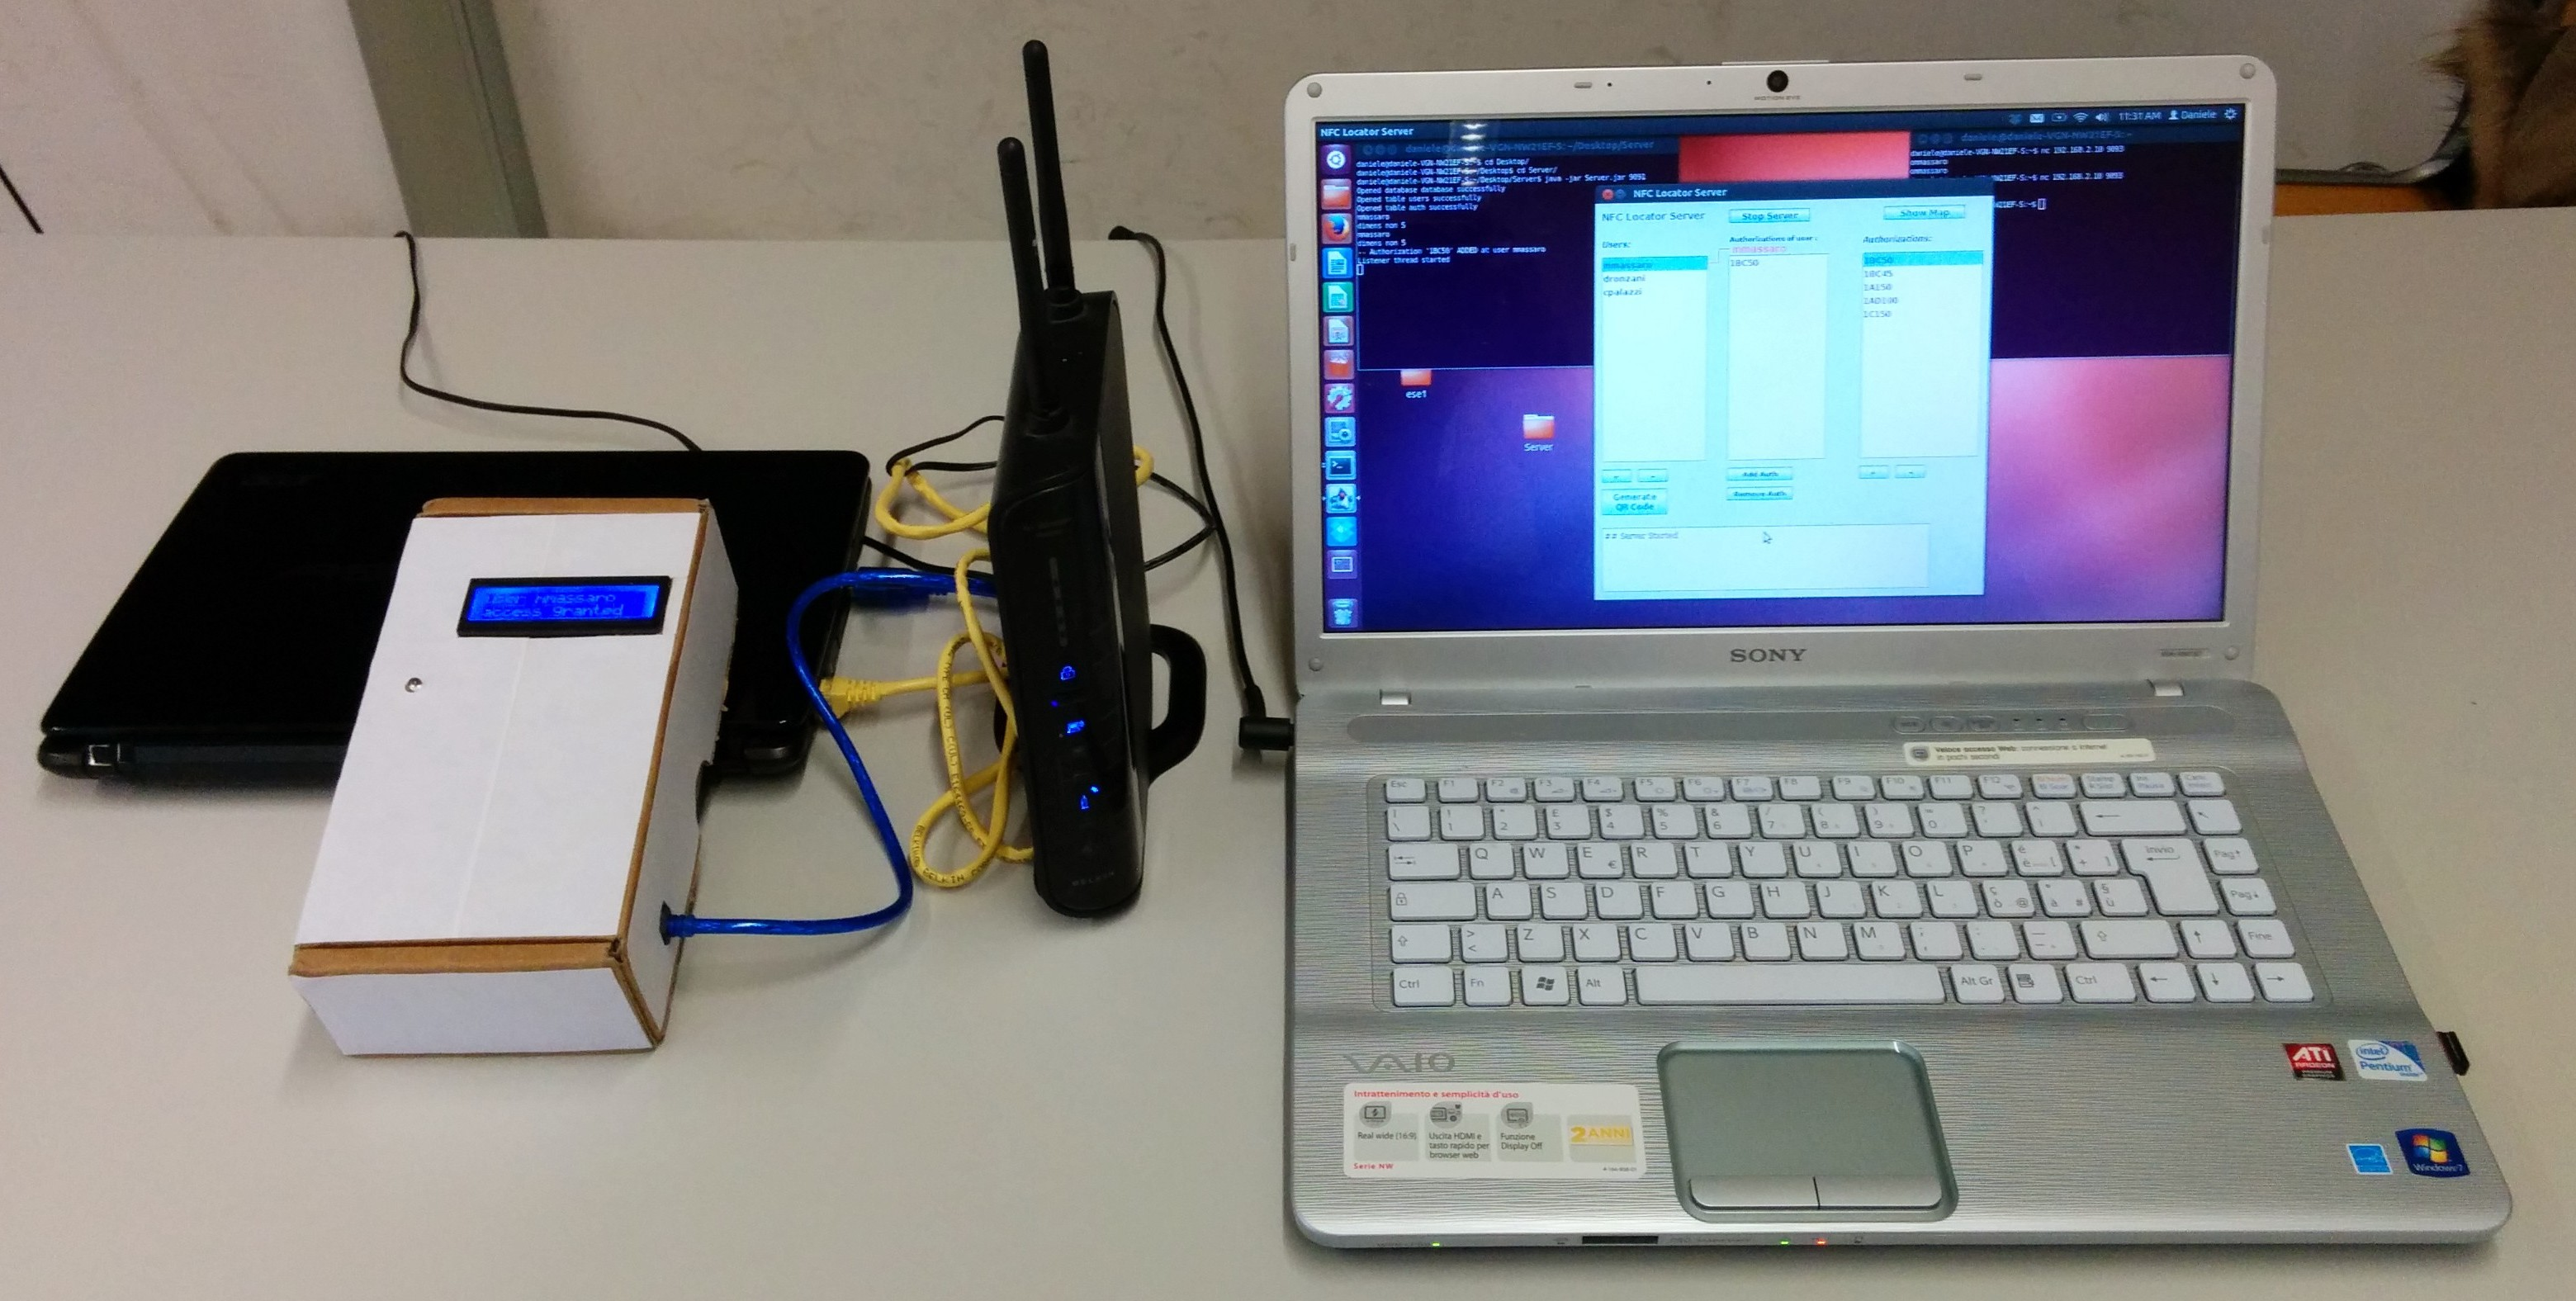
\includegraphics[scale=0.08]{fig8}
\caption{The demonstration platform}
\label{architecture}
\end{figure}

The system introduced here is proposed as a substitute for the current authentication system though NFC tags. The basic idea, which differs from the classical solutions, is the reverse approach of how the user is authenticated: while, in the classical way, the tag represents the access key and the reader is the ``lock'', in our approach the NFC reader of smartphone become the key, and the tag represents the door. In this way, the user does not bring with him the tag, but the reader, that can identify the resource approached and request the access to a remote server.

In addition, the relationship between tag and its resource is inherently a system of localization, because the reading implies physical proximity between the smartphone and the place where the door resides, allowing the system administrator to have an almost real-time view of accesses (and relative positions) of the users during the authentication process.

\subsection{Architecture}
The system is composed by three logical part:
\begin{itemize}
 \item \textbf{Client} (NFC Locator)
 \item \textbf{Server} (NFC Authenticator)
 \item \textbf{Resource} (door’s lock)
\end{itemize}

\begin{figure}[h]
\centering
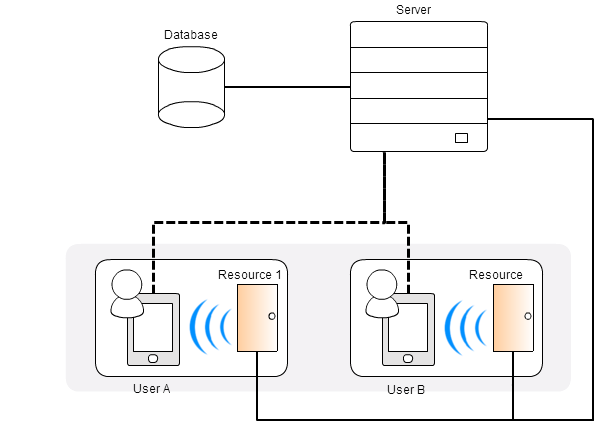
\includegraphics[scale=0.4]{fig1}
\caption{System Architecture}
\label{arch}
\end{figure}

The client consist of an Android application (NFC Locator) that allows the user to detect the resource. After the reading, the app will send the request to access the resource to the remote server.
The server (NFC Authenticator) is an application that receive requests and contains a database that store usernames, passwords, and permission of everyone.  There is also a graphical interface that allows the system administrator to manage the accounts.
The resource consists of a component that can be remotely controlled by the server, in our case a prototype of a door lock. Through an ethernet connection it can communicate on the network with the server and receive the “open” command.

\subsection{Networks}

Three kinds of connections are involved: wired network (between server and resource), wi-fi network (between server and client) and NFC (between client and resource).

The connection between the server and client can happen in two ways that differ regard to safety. The first is the connection via local wi-fi network, in which the smartphone is forced to connect to the local wireless network of the building to gain access to a gate, in fact only in this case can communicate with the control server. The second is the connection to the server using the UMTS mobile telephone technology: in this case the access request travels through the global network, and then get to the server. This mode can only be present if the server has a static external IP address, so that it can be accessed remotely. This second way is much less safer than the first one. For this reason, the connection between client and server is protected with a cryptographic protocol, the Transport Layer Security (TLS), which allows secure communication in the transport layer, preventing eavesdropping or “man in the middle” attacks. 

NFC communication allows data transfer between the client and the resource, in particular a unique identifier representing the door, which will be sent to the server during the authentication process.

\subsection{Client Side}

As said before, the client consist of an Android application that allows to read NFC tags and send information to a remote server.
The application is composed by two parts, the configuration and the reading.

\begin{figure}[h]
\centering
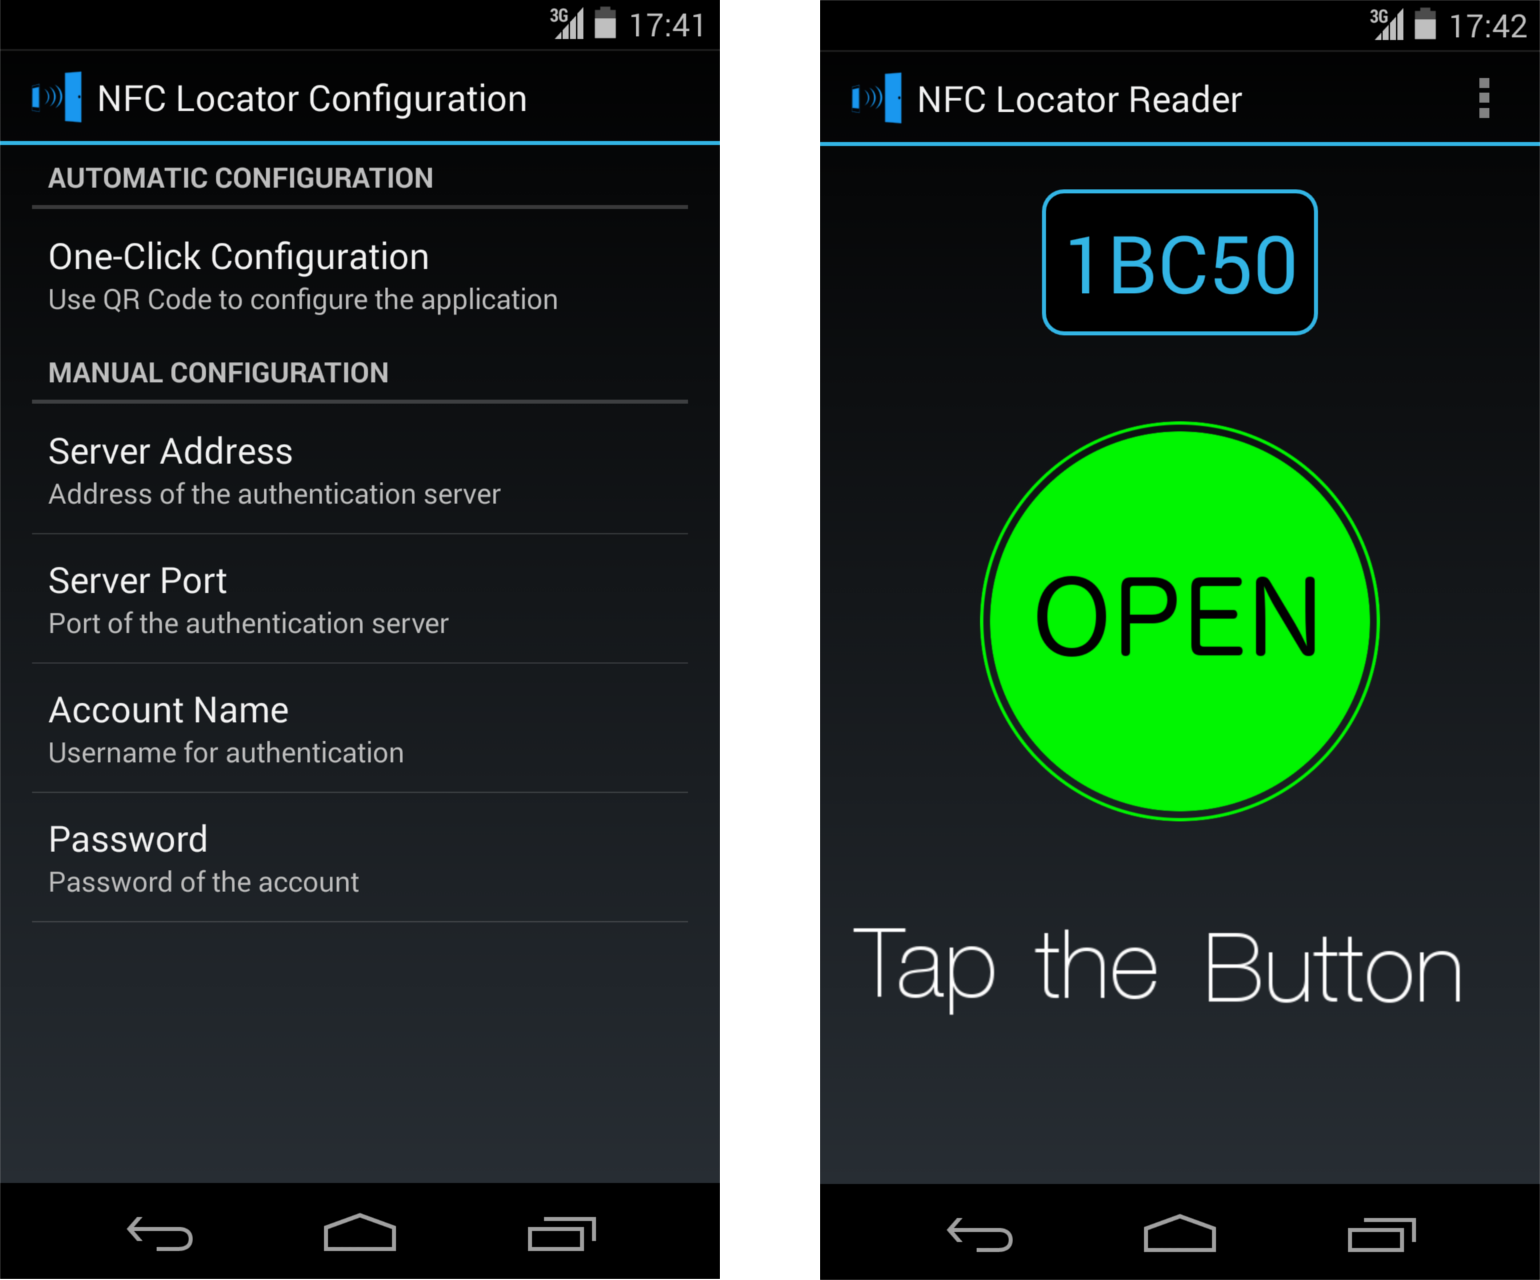
\includegraphics[scale=0.15]{fig2}
\caption{\textbf{NFC Locator: }Left: Configuration window; Right: Reader window}
\label{client}
\end{figure}

\subsubsection{Configuration}

the configuration window allows the user to set all the network parameter and login information, like username and password.
Even if the configuration must be done once, it seemed too difficult to let configure server address and port to an average user, and because the application was made to be user friendly and usable by most people have been added the “One-Click Configuration” option: after an user has been added into the server, can be automatically generated a QR code; the user just have to point the phone to the QR code to setup all network parameter. The protocol used by the QR reader needs a string designed with the following pattern:
\begin{center}
\textit{``address:\textless address\textgreater\ port:\textless port\textgreater\ user:\textless username\textgreater}''
\end{center}


 The only information that have to be inserted manually is the password, for security reason.

\subsubsection{Reading}

to maintain the application easy to use, the user do not have to launch any application to detect a resource. It is enough to approach the phone to the resource to make appear the window on the image 4. The only part that can be touched in the interface is the big green button in the middle, that given it’s large dimension is easily usable even for visually impaired people. When the button is pressed, a request containing the login and the resource ID is sent to the server, while the app shows a progress indicator. The message sent must contains a string in the following pattern:
\begin{center}
\textit{``\textless username\textgreater :\textless password\textgreater :\textless resource ID\textgreater}''
\end{center}
 After a moment the positive or negative response appears. At the end of the operation the window will automatically close, preventing the reiteration of the process. This feature avoid the possibility to open the door while the user is not in the proximity of the lock.

\subsection{Server Side}

The server program is an application that consists of two concurrent entities: one that handles the actual server and one that manages the GUI.

\subsubsection{Listener}

\label{serverCheck}
the server has a listener that waits for messages from clients requesting access to a resource. For this function there is a thread that listens on a port and waits for a TCP/IP communication from the client. The full flow can be seen in Figure 3.
Once the channel is open, the server waits to receive a message from the client containing the user's account information, and the data of tag detected. First, a check is performed on login data received, and only if these are correct is checked that the user has the necessary permission to use the resource. If both controls have a positive outcome, the server open a connection to the requested resource, sending the command to open and possible additional data, such as the username of the requesting user. Only at the reception of the ack by the resource, the server considers the operation completed and sends the positive response to the user.

\begin{figure}[h]
\centering
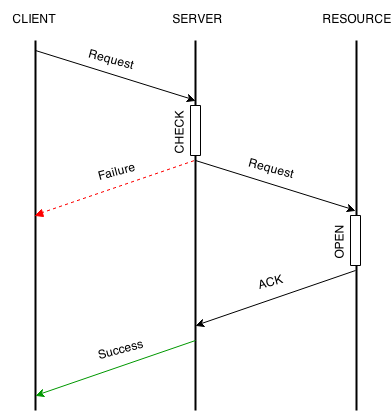
\includegraphics[scale=0.5]{fig3}
\caption{Communication flow}
\label{flow}
\end{figure}

\subsubsection{Graphics}

\begin{figure}[h]
\centering
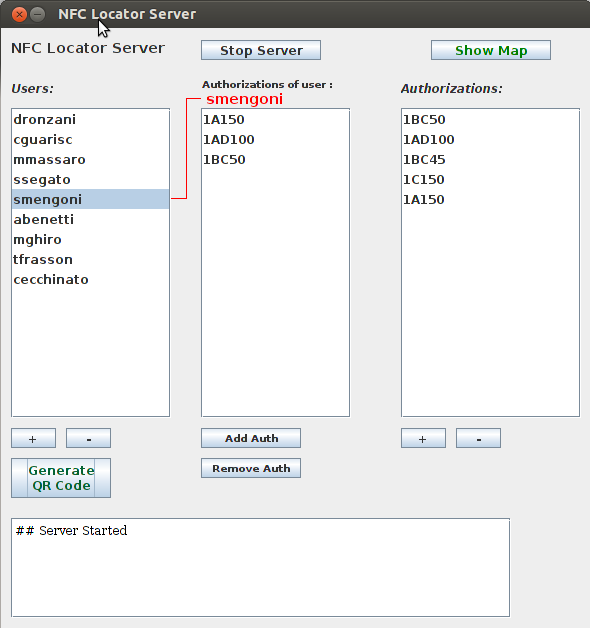
\includegraphics[scale=0.35]{fig4}
\caption{Server GUI}
\label{gui}
\end{figure}

the graphics part is characterized by a window with three main areas:

\begin{itemize}
 \item members list;
 \item authorizations list;
 \item list permissions owned by the user.
\end{itemize}

An element can be added or removed to the user list through the buttons at the bottom. The same applies to the other two lists.
Through the ``Generate QR Code'' button can be created a QR code to automatically configure the client of the selected user.

The ``Start Server'' button starts the listener server to accept requests. From that moment on, every client can connect to the server.

\subsubsection{Map Area}

Another feature is the presence of a window that alerts the administrator of authorized or unauthorized access in a specific location. This window is automatically shown, and display a map of the area (Figure 5a), highlighting the zone in which the user has accessed (Figure 5b), or which has not been authorized (Figure 5c).

\begin{figure}[h]
\centering
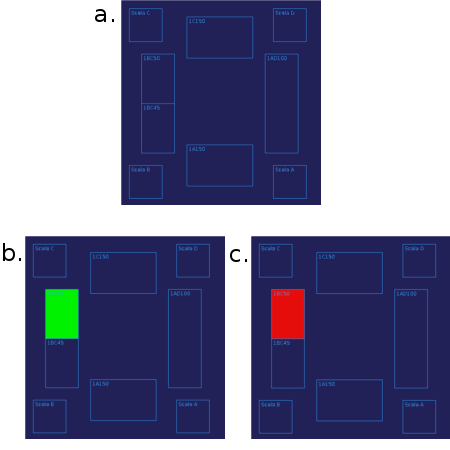
\includegraphics[scale=0.5]{fig5}
\caption{Server map window}
\label{map}
\end{figure}

\subsection{Database}

Users and permissions are stored in a relational database implemented with SQLite [7]. There are three tables. A table contains the information of users: username and password. Another table contains data regarding the resource: name of door and IP:PORT address.
Finally, a third table identifies each pair user-resource to store authorized accesses of each user.
Database has been designed with ER diagram shown in Figure 6.

\begin{figure}[h]
\centering
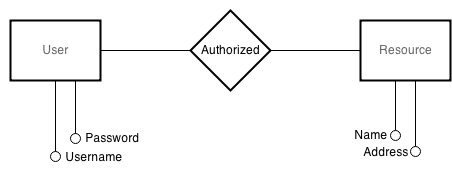
\includegraphics[scale=0.5]{fig6}
\caption{Database ER diagram}
\label{db_ER}
\end{figure}

\subsection{Resource}

\begin{figure}[h]
\centering
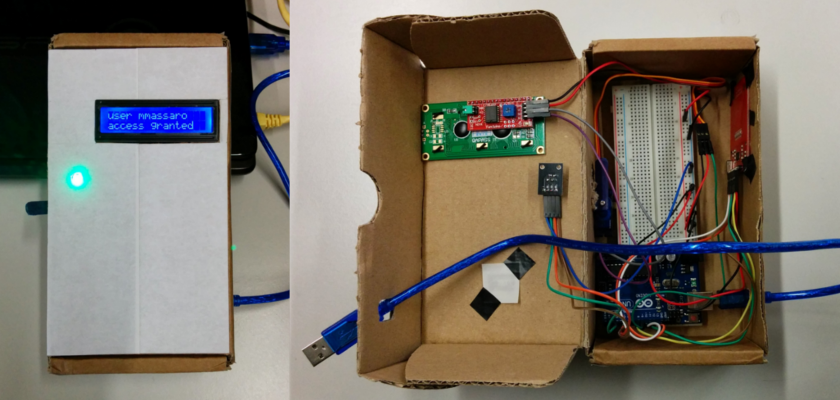
\includegraphics[scale=0.3]{resource}
\caption{Image of the prototype used in the demo}
\label{resource}
\end{figure}

The resource was built to be much similar as possible to a lock. To realize it was used an Arduino Uno r3, programmed to reflect the behaviour of a remotely controlled lock, so there is a small motor that move the closing cylinder and a display that show the state when necessary.
The connection to the server is provided by an ethernet interface, that allow the exchange of packets between them. 
Inside the lock there is an NFC tag, that contains the identification of the resource, needed to be recognised by the server. The tag used is a ``NTAG203'', that contains up to 137 byte of payload.
To preserve the compatibility with cards that are often used now, have been added an RFID reader, also usable in case of emergency or if there are network issues.

\subsection{Usage}

When the whole system is ready, its behavior can be summarized as follow:
\begin{itemize}
 \item a user approach his NFC smartphone to the door lock
 \item the smartphone detect the NFC tag and prompt the user to confirm the operation
 \item when the button on the client window is pressed, the mobile application try to connect to the server, through a TLS connection.
 \item if the connection is successful, the phone sends login and door information to the server
 \item the server verify the information received, and if they are correct the lock will open,  as explained before (\ref{serverCheck})
\end{itemize}

\subsection{Security}

This system was proposed to replace NFC tags, so will be done a comparison between the security offered by both methods.
Tags are passive objects, that can be used even by not authorized users in case of loss. The advantage on the use of a smartphone as user interface is given by the possibility to use a password to unlock it, so it add an obstacle to a possible thief.
A second problem of tags is that they can be read by every reader, even if the tag is not used. For that reason most tag contains encrypted information, or use more sophisticated ways to avoid man in the middle attacks [1].
In the proposed system, the smartphone is the reader, and the only passive entity is the resource, that contains not sensible information (the ID is meaningless outside the system). Moreover, every Android phone turn off the NFC antenna when the screen is locked, preventing possible security issues.
An essential point of the system is represented by the connection between the client and the server, where are exchanged sensible information. For this reason, the connection have been encrypted using the TLS protocol; the client contains a certificate that allow to authenticate the server identity, preventing ``man in the middle'' attacks.
In addition, it is useful to emphasize that in the system there is no authentication data exchanged between the client and the resource. For that reason, even if the NFC communication is eavesdropped, no sensible data can be collected.

\section{Performance}

The system is made to be used very often, so it does not just need to be easy to use, but it must be fast to not annoy users. For this reason have been done tests on the reactivity of the system, and the result are shown of the graph on the Figure 7.

\begin{figure}[h]
\centering
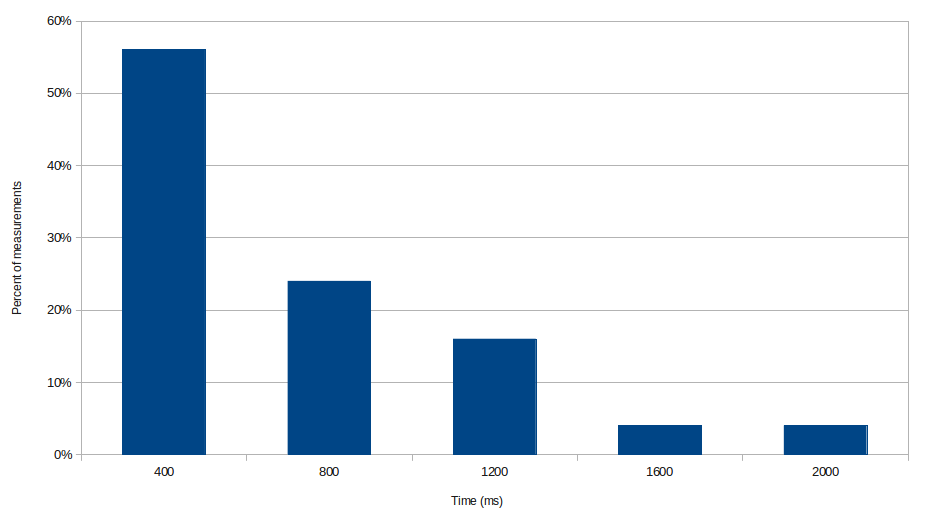
\includegraphics[scale=0.35]{fig7}
\caption{Performance graph}
\label{graph}
\end{figure}

In more than 60\% of the measurements the client completed the communication process in less than 400 ms as can be seen in the cumulative graphic in Figure \ref{graph}.  Sometimes the time can be greater because of network congestions, but the procedure never spends more than a couple of seconds. 
Overall the mean of access time should be lower than the classical approach, because the user does not need to search the NFC card inside the wallet, but have to use his smartphone, that usually is in handy.

\section{Conclusions}

This work has been presented as an alternative to actual NFC authentication systems; have been proposed a new system, that allows to reach a higher security level than some classical RFID card while keeping its simplicity and reactivity, and that makes the key of a real door completely virtual. The virtualization does not just give us the chance to use an Android phone for the authentication, but could also be used to automate all those operations that are now manually handled, like keys/cards distribution: for example a hotel can provide a booking system that sends a QR code through email to customers, allowing them to configure their phone in advance and avoid queue at the reception to gather keys.
Another important feature is the cost of this solution, lower than others [6], in fact all the components used to build the prototype can be bought for less than 30 euros. Moreover, all the elements can be easily assembled without the need of an industrial process, as showed in the demo.


% trigger a \newpage just before the given reference
% number - used to balance the columns on the last page
% adjust value as needed - may need to be readjusted if
% the document is modified later
%\IEEEtriggeratref{8}
% The "triggered" command can be changed if desired:
%\IEEEtriggercmd{\enlargethispage{-5in}}

% references section

% can use a bibliography generated by BibTeX as a .bbl file
% BibTeX documentation can be easily obtained at:
% http://www.ctan.org/tex-archive/biblio/bibtex/contrib/doc/
% The IEEEtran BibTeX style support page is at:
% http://www.michaelshell.org/tex/ieeetran/bibtex/
%\bibliographystyle{IEEEtran}
% argument is your BibTeX string definitions and bibliography database(s)
%\bibliography{IEEEabrv,../bib/paper}
%
% <OR> manually copy in the resultant .bbl file
% set second argument of \begin to the number of references
% (used to reserve space for the reference number labels box)
\begin{thebibliography}{1}

\bibitem{paper1}
Y.S Lee, E. Kim, and M.S. Jung, ``A NFC based Authentication method for defense 
of the Man in the Middle Attack'', in proc. of ICCSIT'2013, Bali, Indonesia, January 2013. 
\bibitem{paper2}
P. Urien, ``NFC Technologies for the Internet Of Things'', Rome, Italy, June, 2013.
\bibitem{paper3}
E. Haselsteiner and K. Breitfuss, ``Security in Near Field Communication (NFC), Strengths and Weaknesses'' 
Gratkorn, Austria, July 2006.
\bibitem{paper4}
G. Van Damme and K. Wouters, ``Practical Experiences with NFC Security on mobile Phones'',
Workshop on RFID Security, 2009.
\bibitem{paper5}
W. Chen, G.P. Hancke, K.E. Mayes, Y. Lien, and J-H. Chiu, ``NFC Mobile Transactions and Authentication based on GSM Network'', 
Monaco, Germany, April 2010.
\bibitem{paper6}
P. Urien, ``A Secure Cloud of Electronic Keys for NFC Locks Securely Controlled by NFC Smartphones'',
in proc. of IEEE CCNC Las Vegas, US, January 2014.
\bibitem{sqlite}
SQLite Homepage, http://www.sqlite.org
\bibitem{nfc}
NFC Forum Specifications, http://www.nfc-forum.org/specs/
\end{thebibliography}




% that's all folks
\end{document}


